%%%%%%%%%%%%%%%%%%%%%%%%%%%%%%%%%%%%%%%%%%%%%%%%%%%
%																													
%																												
%																													
%									Importations	de bibliothèques	
%																													
%																												
%%%%%%%%%%%%%%%%%%%%%%%%%%%%%%%%%%%%%%%%%%%%%%%%%%%


\documentclass[hidelinks]{article}
\usepackage[utf8]{inputenc}
\usepackage{graphicx}
\usepackage[T1]{fontenc}
\usepackage[french]{babel}
\usepackage{csquotes}
\usepackage[section]{placeins}
\usepackage{tikz}
\usepackage{hyperref}
\usepackage{afterpage}
\usepackage{pdfpages}
\usepackage{wrapfig}
\usepackage{amsmath, mathtools}
\usepackage{amssymb}
\usepackage{fancyhdr}
\usepackage[all]{background}


%%%%%%%%%%%%%%%%%%%%%%%%%%%%%%%%%%%%%%%%%%%%%%%%%%%%%%%%%%%%%%%%%%%%
%																																	   %
%																																	   %
%																																	   %
%															Page de garde															   %
%																																	   %
%																																	   %
%%%%%%%%%%%%%%%%%%%%%%%%%%%%%%%%%%%%%%%%%%%%%%%%%%%%%%%%%%%%%%%%%%%%



\newcommand{\MyGraphicLogo}{% For imported graphic logo
\begin{tikzpicture}[remember picture,overlay,yshift=-15cm, xshift=10.5cm]
	\definecolor{gris}{RGB}{16,52,78}
	\definecolor{jaune_fonce}{RGB}{0, 107, 163}
	\definecolor{jaune}{RGB}{0, 151, 136}
	\fill [gris] (-10.5,-10) -- (0,-4.5) -- (14,-13) -- (14,-16)--(0,-16)--(-10.5,-16);
	\fill [jaune_fonce] (0,-4.5) -- (-10.5,-10) -- (-10.5, 1.8);
	\node at (3.8,0.4) {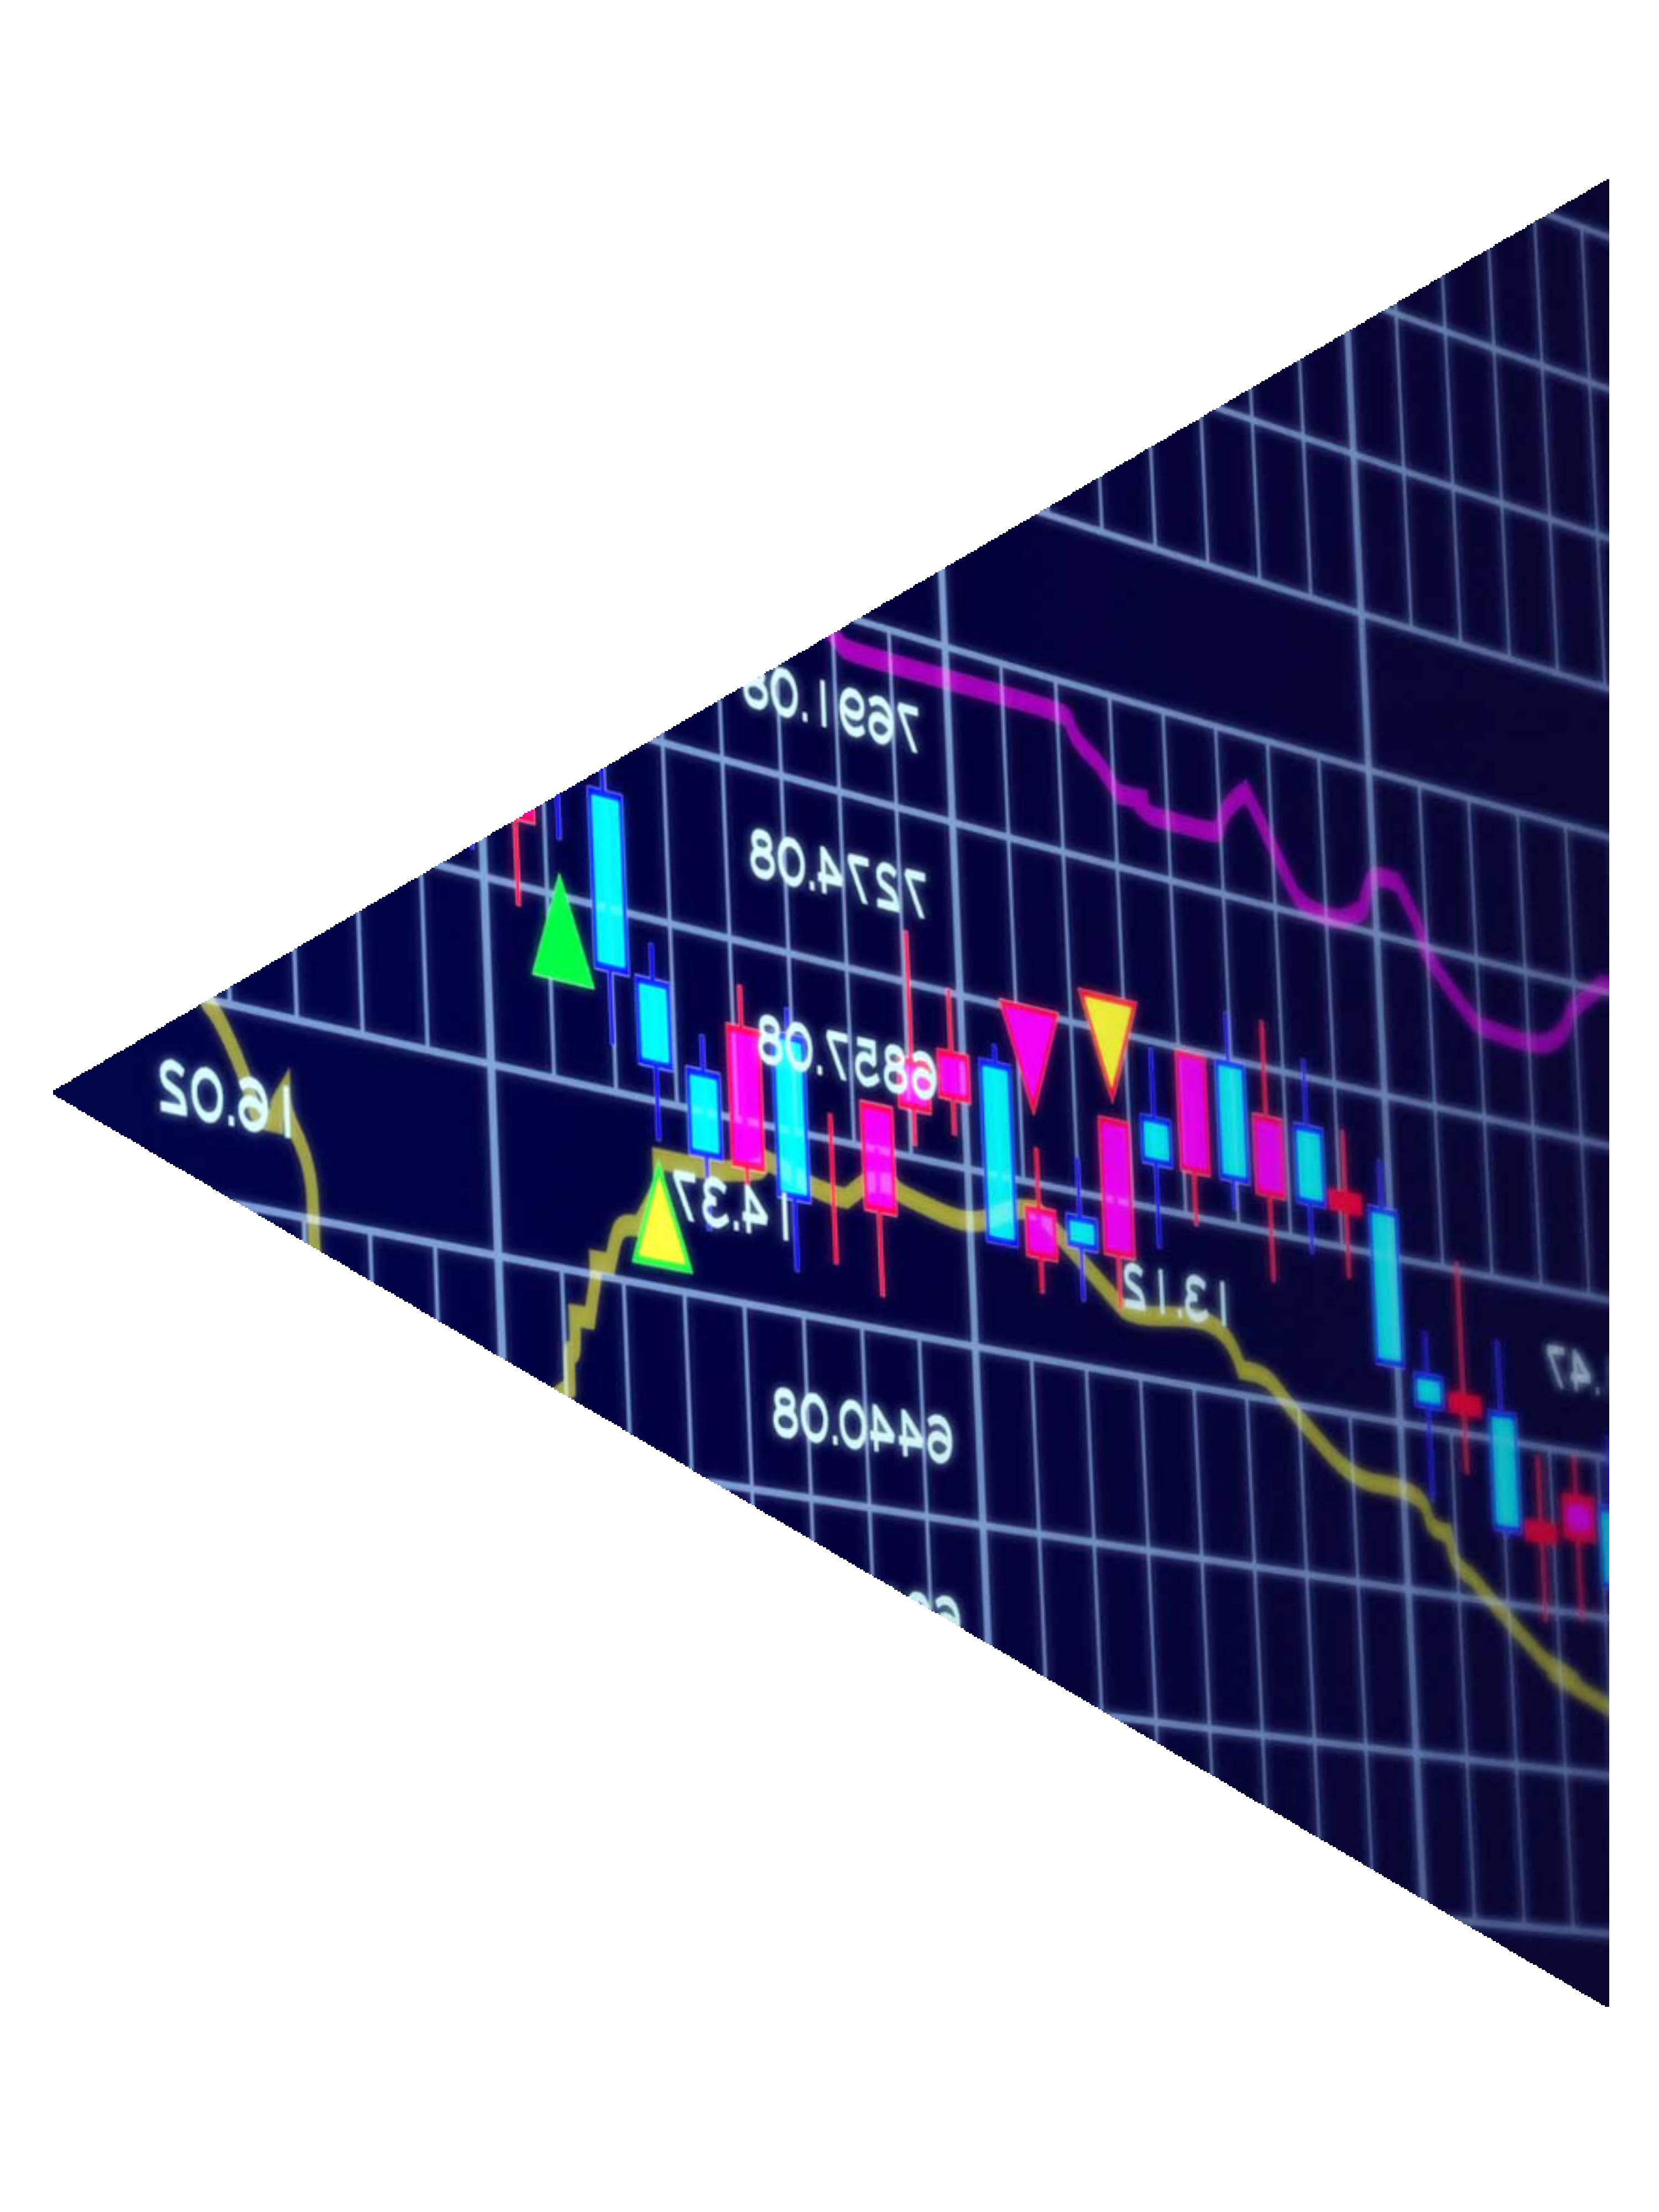
\includegraphics[width=22cm]{triangle.png}};
	\fill [jaune] (14,5) -- (2.5, 12) -- (20,25) -- (14, 20);
 \end{tikzpicture}}


\SetBgContents{\MyGraphicLogo}% Select included image

\SetBgPosition{current page.north west}% Select location
\SetBgOpacity{1.0}% Select opacity
\SetBgAngle{0.0}% Select roation of logo
\SetBgScale{1.0}% Select scale factor of logo



%%%%%%%%%%%%%%%%%%%%%%%%%%%%%%%%%%%%%%%%%%%%%%%%%%%%%%%%%%%%%%%%%%%%
%																																	   %
%																																	   %
%																																	   %
%										Informations générales sur le document															   %
%																																	   %
%																																	   %
%%%%%%%%%%%%%%%%%%%%%%%%%%%%%%%%%%%%%%%%%%%%%%%%%%%%%%%%%%%%%%%%%%%%

 \usepackage{fontspec}
  \usepackage[bold-style=upright]{unicode-math}
  \defaultfontfeatures{Scale=1}
  \setmainfont[Ligatures=TeX,Numbers=OldStyle]{Lucida Bright OT}
  \setmathfont[RawFeature=+ss04]{Lucida Bright Math OT}
  \setsansfont[Scale=1.0,Numbers=OldStyle]{Myriad Pro}
  \newfontfamily\fullcaps[Letters=Uppercase,Numbers=Uppercase]{Myriad Pro}
  \usepackage[babel=true]{microtype}
  \usepackage{icomma}
  
  
  
  
  
  
  
  
  
  
  
\title{Binomial pricing formula}
\author{Maxence COUPET - \href{mailto:maxence.coupet@gmail.com}{maxence.coupet@gmail.com}}
\date{March 2018}



\MHInternalSyntaxOn
\MH_set_boolean_T:n {outer_mult}
\MHInternalSyntaxOff

\newenvironment{nalign}{
    \begin{equation}
    \begin{aligned}
}{
    \end{aligned}
    \end{equation}
    \ignorespacesafterend
}
%%%%%%%%%%%%%%%%%%%%%%%%%%%%%%%%%%%%%%%%%%%%%%%%%%%%%%%%%%%%%%%%%%%%
%																																	   %
%																																	   %
%																																	   %
%												Mis en page du document																   %
%																																	   %
%																																	   %
%%%%%%%%%%%%%%%%%%%%%%%%%%%%%%%%%%%%%%%%%%%%%%%%%%%%%%%%%%%%%%%%%%%%


\begin{document}
	\selectlanguage{french}
	% page de garde
	\pagenumbering{gobble}
	\maketitle
	\newpage
	% début du rapport
	
	
	


\newcommand{\MyGraphicLog}{% For imported graphic logo
\begin{tikzpicture}[remember picture,overlay,yshift=-15cm, xshift=10.5cm]
\definecolor{jaune}{RGB}{16, 52, 78};
\fill[jaune] (-11, -16) -- (13, -16) -- (13, -12.1) -- (-11, -12.1);
 \end{tikzpicture}}


\SetBgContents{\MyGraphicLog}% Select included image


\SetBgPosition{current page.north west}% Select location
\SetBgOpacity{1.0}% Select opacity
\SetBgAngle{0.0}% Select roation of logo
\SetBgScale{1.0}% Select scale factor of logo

\pagestyle{fancy}
\renewcommand\headrulewidth{0pt}
\lhead{}\chead{}\rhead{}
\cfoot{\vspace*{6\baselineskip} \textcolor{white}{\thepage} \large}
	\newpage

	\pagenumbering{arabic}

%%%%%%%%%%%%%%%%%%%%%%%%%%%%%%%%%%%%%%%%%%%%%%%%%%%%%%%%%%%%%%%%%%%%
%																																	   %
%																																	   %
%																																	   %
%								Début du document (commencez à taper votre texte ici)													   %
%																																	   %
%																																	   %
%%%%%%%%%%%%%%%%%%%%%%%%%%%%%%%%%%%%%%%%%%%%%%%%%%%%%%%%%%%%%%%%%%%%

	The main idea behind binomial pricing for a derivative is to consider that at one point in time, the underlying price can only moove in two direction : up or down. We will use the following notation : $S_0$ is the underlying price, $T$ is the maturirty of the derivative, $f$ is the fair price of the derivative, $f_u$ is the price of the derivative after an upward movement and $f_d$ is the price of the derivative after a downward movement, $r$ is the risk-free rate, $u$ is the muliplicative rate of the underlying for an upward movement (the price after an upward movement is then $S_0 u$), $d$ is the multiplicative rate of the underlying for an downward movement and $p$ the probability of an upward movement.
	
	For this document, we will only consider the one period model, which means that we consider that at time $t=0$, the underlying price is $S_0$ and at time $t=T$ the underlying price can only be $S_0u$ or $S_0d$. Figure \ref{fig:binom} summarize the one step binomial model. Even if the one step binomial model is too simple to give a good approximation of the price of a derivative, a multi steps binomial method is very accurate and one can even show the the price of the mutli steps binomial method converges to the Black-Scholes price. Thus the binomial pricing method is a discret version of the Black-Scholes formula and one can see a multi steps binomial method as a succession of one step binomial method, therefore the formula for a one step binomial method can be generalized.
	
\begin{figure}[!h]
	\centering
	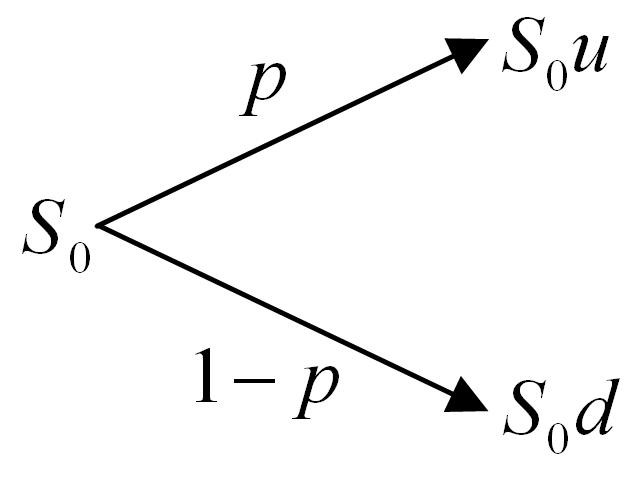
\includegraphics[width=0.3\textwidth]{binomial.jpg}
    \caption{One-step binomial tree pricing method}
    \label{fig:binom}
    \end{figure}

	
	Let's consider a portfolio with a short position in the derivative and a long position in $\Delta$ underlyings (eventually, if $\Delta<0$, we will take a short postion of $|\Delta|$ underlyings). The value of our portfolio will thus be $\Delta S_0 - f$ at $t=0$, $\Delta S_0 u - f_u$ at time $t=T$ after an upward movement and $\Delta S_0 d - f_d$ at time $t=T$ after an downward movement.
	
	We want our portfolio to be risk-free, which means that we want to be sure of his value a time $t=T$, so the value after an upward and downward movement should equal and we have :
	\begin{nalign}
	\Delta S_0 u - f_u = \Delta S_0 d - f_d \Rightarrow \Delta = \frac{f_u - f_d}{S_0 (u-d)}
	\end{nalign}
	
	We now have an analytic formula for the $\Delta$. Since our portfolio is risk-free, its return should not be higher or lower than the risk-free rate, otherwise there would be an arbitrage to perform. The arbitrage-free condition allow use to write that the value of the portfolio at time $t=0$ should be equal to the value of the portfolio at time $t=T$ (the upward or dorward value, remember that they are equal), discounted with the risk-free rate. We then have :
	
	\begin{nalign}
	\Delta S_0 - f = e^{-rT}(\Delta S_0 u - f_u)
	\end{nalign}
	
	By combining this equation to the analytic formula for $\Delta$, we can now proove the binomial model pricing formula :
	
	\begin{nalign}
	f &= \Delta S_0 - e^{-rT}\Delta S_0 u + e^{-rT}f_u \\
	&= \Delta S_0 \left( 1 - u e^{-rT} \right) + e^{-rT}f_u \\
	&= S_0 \frac{f_u - f_d}{S_0 (u-d)}\left( 1 - u e^{-rT} \right) + \frac{e^{-rT}f_u(u-d)}{u-d} \\
	&= \frac{f_u \left(1 - ue^{-rT} + ue^{-rT} - de^{-rT}\right) + f_d \left(ue^{-rT}-1\right)}{u-d} \\
	&= f_u \frac{1 - de^{-rT}}{u-d} + f_d \frac{ue^{-rT}-1}{u-d} \\
	&= e^{-rT} \left( f_u \frac{e^{rT} - d}{u-d} + f_d \frac{u-e^{rT}}{u-d}  \right)
	\end{nalign}
	
	Let $p=\frac{e^{rT} - d}{u-d} $, we also note that $1-p = \frac{u-e^{rT}}{u-d}$. Therefore, we have :
	\begin{nalign}
	f= e^{-rT} \left[ p f_u + (1-p) f_d   \right]
	\end{nalign}
	
	Now the only unknown parameters are $u$ and $d$. We have an arbitrage-free condition on those parameters :
	
	\begin{nalign}
		0<d<e^{rT}<u
	\end{nalign}
	
	Otherwise, one could take advantage of the market with an arbitrage and the pricing will not be a good representation of the market.
	
	We will define $u$ and $d$ as a function of the volatility of the underlying. It is important to remember that the volatility of the return of an underlying following a log-normal law (the geometric Brownian motion) is $\sigma \sqrt{T}$ and that the formula giving the variance for a random variable $X$ is : $Var(X)=\mathbb{E}(X^2)- \mathbb{E}(X)^2$.
	
	Let's consider consider the one-step binomial model, on the period of length $T$, we have a probability $p$ that the return will be $u-1$ and a probability $1-p$ that the return will be $d-1$. The variance is therfore :
	$$Var = p(u-1)^2+(1-p)(d-1)^2-\left[p(u-1)+(1-p)(d-1) \right]^2$$
	
	Combining what we know about the volatility of the returns with the above formula will lead to :
	$$pu^2 + (1-p)d^2 - \left[pu+(1-p)d\right]^2 = \sigma^2 \sqrt{T}$$
	
	Now we use the explicit formula for $p$ in the previous equation and present the equation that any $u$ and $d$ must respect :
	
	\begin{nalign}
		e^{rT}(u+d) -ud - e^{2rT} = \sigma^2 \sqrt{T}
	\end{nalign}
	
	Cox, Ross and Rubenstein proposed one solution for this equation, which is recombining ($ud=1$) and very popular :
	
	\begin{nalign}
		&u = e^{\sigma \sqrt{T}} \\
		&d =  e^{-\sigma \sqrt{T}}
	\end{nalign}
\end{document}